\documentclass[final,5p,times,twocolumn]{elsarticle}

\usepackage{algorithm}
\usepackage{amsmath}
\usepackage{graphicx}
\usepackage{hyperref}
\usepackage{siunitx}  % use \si{\angstrom} for Angstrom
\usepackage{subcaption} % use \subfigure
\usepackage{xspace}

\newcommand{\pygbe}{\texttt{PyGBe}\xspace}
\newcommand{\gmres}{\textsc{gmres}\xspace}
\newcommand{\bem}{\textsc{bem}\xspace}
\newcommand{\fmm}{\textsc{fmm}\xspace}
\newcommand{\kifmm}{\textsc{kifmm}\xspace}
\newcommand{\ncrit}{n_{\mathrm{crit}}}  % number of particles per leaf
\newcommand{\ses}{\textsc{ses}\xspace}
\newcommand{\msms}{\texttt{\textsc{msms}}\xspace}
\newcommand{\ie}{\textit{i}.\textit{e}., }

\graphicspath{{figs/}}

\journal{Computer Physics Communications}
\begin{document}

\begin{frontmatter}
\title{High-productivity, high-performance workflow for virus-scale electrostatic simulations with Bempp-Exafmm}

\author[gwu]{Tingyu Wang}
\ead{twang66@gwu.edu}

\author[usm]{Christopher D. Cooper}
\ead{christopher.cooper@usm.cl}

\author[ucl]{Timo Betcke}
\ead{t.betcke@ucl.ac.uk}

\author[gwu]{Lorena A. Barba}
\ead{labarba@gwu.edu}

\address[gwu]{Department of Mechanical and Aerospace Engineering, The George Washington University, Washington DC}
\address[usm]{Department of Mechanical Engineering and Centro Cient\'ifico Tecnol\'ogico de Valpara\'iso, Universidad T\'ecnica Federico Santa Mar\'ia, Valpara\'iso, Chile}
\address[ucl]{Department of Mathematics, University College London, UK}

%% abstract
\begin{abstract}
    % Maybe add a sentence to describe the importance of molecular electrostatics simulations.
    We present a high-productivity and high-performance Poisson-Boltzmann (PB) solver based on Exafmm, a fast multipole method (FMM) library and Bempp, a Galerkin boundary element method (BEM) package.
    Bempp-Exafmm tightly incorporates an easy-to-use Python interface into the well optimized computation kernels that are written in compiled languages.
    Thanks to Python's rich ecosystem in scientific computing, users can perform PB simulations interactively via Jupyter notebooks, and thus it opens up the possibility for faster prototyping and analyzing.
    To showcase the capability of our software, we computed the solvation free energies of various biomolecular structures, including Zika virus.
    We were able to compute the solvation energy of Zika virus with 10 million boundary elements in 80 minutes on a single node.
    In addition, we present the verification results of Bempp-Exafmm in a grid convergence study, and demonstrate how its flexibility and ease of use facilitate the comparison of different boundary integral formulations in terms of conditioning, convergence and solution time.
\end{abstract}

%% keyword
\begin{keyword}
    boundary integral equation \sep boundary element method \sep Galerkin method \sep fast multipole method \sep
    Python \sep biomolecular electrostatics \sep implicit solvent \sep Poisson-Boltzmann \sep solvation free energy
\end{keyword}

\end{frontmatter}

% body of paper
\section{Introduction}\label{sec:intro}
%!TEX root = main.tex
Electrostatics plays a key role in the structure and function of biological molecules.
Long-range electrostatic effects intervene in various essential processes, such as protein binding, with biomolecules always present in a solution of water with ions.
Computer simulations to study electrostatic interactions in biomolecular systems divide into those that represent the solvent explicitly---in full atomic detail---or implicitly.
In so-called implicit-solvent models~\cite{RouxSimonson1999,DecherchiETal2015}, the solvent degrees of freedom are averaged out in a continuum description.
Starting from electrostatic theory, this leads to a mathematical model based on the Poisson-Boltzmann equation, and widely used to compute mean-field electrostatic potentials and solvation free energies.
Poisson-Boltzmann solvers have been numerically implemented using finite difference \cite{RocchiaAlexovHonig2001, BakerETal2001}, finite element \cite{BakerETal2001,BondETal2010,HolstETal2012}, boundary element \cite{AltmanBardhanWhiteTidor2009, GengKrasny2013, ZhangPengHuangPitsianisSunLu2015, CooperBardhanBarba2014}, and (semi) analytical \cite{LotanHead-Gordon2006,FelbergETal2017} methods, scaling up to problems as large as virus capsids \cite{ZhangETal2019,MartinezETal2019}.

Virus-scale simulations are at the limit of what can be accomplished in computational biophysics, using leadership computing facilities.
The first explicit-solvent atomic simulation of a virus using molecular dynamics was published just 15 years ago, modeling a plant virus (satellite tobacco mosaic virus) of 1.7 nm in diameter \cite{FreddolinoETal2006}.
The full model included 1 million atoms, and the computations ran for many days on the world-class facilities at the National Center for Supercomputing Application (NCSA), University of Illinois.
Using largely the same methods, researchers just last year could model the full viral envelope of a 2009 pandemic influenza A H1N1 virus, with a diameter of about 115 nm \cite{DurrantETal2020}.
In this case, the full system consisted of 160 million atoms, and the computations ran on the Blue Waters supercomputer at NCSA using 115k processor cores (4,096 physical nodes).
This is among the largest biomolecular systems ever simulated using all-atom molecular dynamics.

Only a few elite researchers can access these leadership computing facilities, however, and if molecular science of viruses is to progress, computational tools that are more widely accessible are needed.
The vision behind this paper is to build an electrostatic simulation platform for biomolecular applications that allows researchers to access it via the Python/Jupyter ecosystem. This provides a high degree of flexibility in the underlying formulations, rapid prototyping of novel models, ease of deployment and integration into existing simulation workflows.

To achieve this vision, we are coupling two libraries, the high-level Galerkin boundary element library Bempp, which is fully developed in Python, and the very fast low-level high-performance fast multipole method (\fmm) library Exafmm. 
Boundary integral problems are described in Bempp using a high-level approach that enables building even complex block-operator systems in just a few lines of Python code. Bempp then executes the discretization, depending on the chosen parameters and machine environment. 
Exafmm is called as a matrix-vector black-box below the user level, hiding all technicalities associated with the discretization.

This approach has the following advantages as compared to an integrated PB solver implemented in, for example, C++:
\begin{itemize}
	\item \textit{Strict separation of concerns}. The user-level description of the electrostatic problem is completely separated from the underlying discretization routines and the \fmm coupling. One can easily move between different types of implementations (e.g., dense discretization, \fmm) editing a single parameter, change input file handling or postprocessing.
	\item \textit{Fast prototyping of different formulations}. We present in this paper results produced with a direct formulation and derivative or Juffer-type formulations. Applying these different formulations requires editing just a few lines of high-level code. The user can easily experiment with other models, such as piecewise solvation models with different solvation parameters in each layer.
	\item \textit{Portability}. Bempp and Exafmm can easily be installed as a joint Docker image that is automatically tracking the current development of these libraries. The whole solution workflow can be implemented in a brief Jupyter notebook.
\end{itemize}
A high-level productive approach does come with some costs. A dedicated highly specialized C++ code that integrates all steps might be faster than our solution. Nevertheless, in this paper we demonstrate that our software platform is highly competitive for real-world solvation energy computations (and many other electrostatic computations), while preserving full flexibility through the use of a high-productivity Python environment.

We present results that show the power of interactive computing to study modeling variations, results to confirm code correctness and describe performance, and a final showcase that computes solvation free energy for a medium-sized virus particle.
Our first result explains the behavior of two solution methods that vary in whether they solve for the potential internal or external to the molecular interface, from the conditioning point of view.
Solution verification via grid-convergence studies with two problem set-ups gives us confidence in the software implementation.
Performance-wise, we show results with problem sizes up to 2 million boundary elements, we show computational complexity of the \fmm evaluations, and timing breakdowns of the solver.
The final result uses a realistic structure, the enveloped Zika virus, computing the surface potential and solvation free energy with about 10 million boundary elements.
All results are reproducible and we share scripts, data, configuration files, and Jupyter notebooks in the manuscript repository, found at \url{https://github.com/barbagroup/bempp_exafmm_paper/}, in addition to permanent archives in Zenodo.
Permanent identifiers are provided at the end of the Results section.


\section{Methods}\label{sec:methods}
\subsection{A boundary integral formulation of electrostatics in molecular solvation}

We showcase our development by modeling molecular solvation with the so-called implicit-solvent model \cite{RouxSimonson1999,DescherchiETal2015}. 
As sketched in Figure XX, this model represents a dissolved molecule as a solute-shaped cavity ($\Omega_1$) inside an infinite medium ($\Omega_2$), where we can apply continuum electrostatic theory.
Then, we can compute the change in electrostatic potential as we charge up the cavity with the solute's partial charges, represented as a collection of Direc-delta functions.
The solvent ($\Omega_2$) usually consists of water ($\epsilon_2\approx$80) with salt, which is pushed around by the electric field. 
At equilibrium, the salt ions arrange according to a Boltzmann distribution, and if we consider them as point charges, this is well modeled by the linearized Poisson-Boltzmann equation. 
On the other hand, the electrostatics in the solute cavity behaves according to the Poisson equation in a low dielectric medium ($\epsilon_1\approx$2---4), forced by the solute's point charges.
These two equations are interfaced on the molecular surface ($\Gamma$), where the potential and electric displacement must be continuous.
The resulting system of partial differential equations is
%
\begin{align} \label{eq:pde}
\nabla^2\phi_1 &= \frac{1}{\epsilon_1}\sum_k q_k\delta(\mathbf{r},\mathbf{r}_k) \text{ in the solute ($\Omega_1$),}\nonumber\\
(\nabla^2-\kappa^2)\phi_2 &= 0 \text{ in the solvent ($\Omega_2$),}\nonumber\\
\phi_1 &= \phi_2 \quad \epsilon_1\frac{\partial \phi_1}{\partial\mathbf{n}} = \epsilon_2\frac{\partial \phi_2}{\partial\mathbf{n}} \text{ on the interface ($\Gamma$)}.
\end{align}
%
where $\Omega_1$ and $\Omega_2$ are the solute and solvent regions, respectively, interfaced by the molecular surface $\Gamma$.
There are several available definitions for $\Gamma$, such as van der Waals, solvent accessible (SAS), solvent excluded (SES), and Gaussian surfaces \cite{HarrisFenley2013}, however, in this work we use the SES.

Equation \eqref{eq:pde} can be represented as an integral equation running over $\Gamma$ by using Green's second identity, yielding
%
\begin{align} \label{eq:volume_potential}
\phi_{1}+ K_{L}^{\Omega_1}(\phi_{1,\Gamma}) -  V_{L}^{\Omega_1} \left(\frac{\partial}{\partial \mathbf{n}}  \phi_{1,\Gamma}  \right) & = \frac{1}{\epsilon_1} \sum_{k=0}^{N_q}  \frac{q_k}{4\pi|\mathbf{r}_{\Omega_1} - \mathbf{r}_k|}  \quad \text{on $\Omega_1$,} \nonumber \\
\phi_{2} - K_{Y}^{\Omega_2}(\phi_{2,\Gamma}) + V_{Y}^{\Omega_2} \left( \frac{\partial}{\partial \mathbf{n}} \phi_{2,\Gamma} \right) & = 0 \quad \text{on $\Omega_2$,}
\end{align}
%
where $\phi_{1,\Gamma} = \phi_1(\mathbf{r}_\Gamma)$ and $\phi_{2,\Gamma} = \phi_2(\mathbf{r}_\Gamma)$ evaluated at $\Gamma$ approaching from $\Omega_1$ and $\Omega_2$, respectively. $K$ and $V$ are the double- and single-layer potentials from Equation XX, for the Laplace and modified Helmholtz (Yukawa) kernel. 
We can use Equation \eqref{eq:volume_potential} to compute $\phi_\Gamma$ and $\partial\phi_\Gamma/\partial\mathbf{n}$ with either the \emph{direct} or \emph{Juffer} formulations.
The simpler direct formulation is a result of evaluating $\phi_1$ and $\phi_2$ in the limit as $\mathbf{r}$ approaches $\Gamma$, and applying the interface conditions from Equation \eqref{eq:pde}, giving
%
\begin{align} \label{eq:direct}
\frac{\phi_{1,\Gamma}}{2}+ K_{L}^{\Gamma}(\phi_{1,\Gamma}) -  V_{L}^{\Gamma} \left(\frac{\partial}{\partial \mathbf{n}}  \phi_{1,\Gamma}  \right) & = \frac{1}{\epsilon_1} \sum_{k=0}^{N_q}  \frac{q_k}{4\pi|\mathbf{r}_{\Gamma} - \mathbf{r}_k|} \nonumber \\
\frac{\phi_{1,\Gamma}}{2} - K_{Y}^{\Gamma}(\phi_{1,\Gamma}) + \frac{\epsilon_1}{\epsilon_2}V_{Y}^{\Gamma} \left( \frac{\partial}{\partial \mathbf{n}} \phi_{1,\Gamma} \right) & = 0
\end{align}
%
Unfortunately, this formulation is ill-conditioned, as the condition number of the resulting matrix grows with the number of discretization elements. 
A better conditioned formulation was derived by Juffer \emph{et al.} \cite{JufferETal1992}, where they took the normal derivative of Equation \eqref{eq:potential_volume}, and couple both $\phi$ and $\partial\phi/\partial\mathbf{n}$ on the boundary as follows
%
\begin{equation}\label{eq:juffer}
\end{equation}

As we charge up the cavity, the solvent will react due to polarization and rearrangement of the salt ions. 
We call the electrostatic potential resulting from this solvent effect a \emph{reaction} potential ($\phi_{reac}$), and we can write the following decomposition in $\Omega_1$ 
%
\begin{equation}
\phi_1 = \phi_{reac} + \phi_{coul}
\end{equation}
%
where $\phi_{coul}$ is the Coulombic potential from the solute point charges only.
Having $\phi_{1,\Gamma}$ and $\partial\phi_{1,\Gamma}/\partial\mathbf{n}$ from Equation \eqref{eq:direct} or Equation \eqref{eq:juffer}, we can compute $\phi_{reac}$ by substracting out the Coulombic contribution in the right-hand side of Equation \eqref{eq:potential_volume}
%
\begin{equation}\label{eq:phi_reac}
\phi_{reac} = -K_{L}^{\Omega_1}(\phi_{1,\Gamma}) +  V_{L}^{\Omega_1} \left(\frac{\partial}{\partial \mathbf{n}}  \phi_{1,\Gamma}  \right) 
\end{equation}

The work required to dissolve a molecule, known as solvation free energy, is usually divided into nonpolar and polar components.
The nonpolar part generates the empty solute-shaped cavity in the solvent, which is later charged by placing the partial charges inside the cavity, giving rise to a polar term in the energy. 
The work in placing the partial charges is performed under $\phi_{reac}$, and it can be computed as
%
\begin{equation} \label{eq:energy}
\Delta G^{polar}_{solv} = \frac{1}{2}\int_{\Omega_1} \rho\phi_{reac}d\mathbf{r} = \frac{1}{2}\sum_{k=1}^{N_q}q_k\phi_{reac}(\mathbf{r}_k)
\end{equation}

%!TEX root = main.tex
\subsection{An introduction to Bempp}
Bempp \cite{Betcke2021} is a Python based boundary element library for the Galerkin discretization of boundary integral operators in electrostatics, acoustics and electromagnetics.
Bempp originally started as mixed Python/C++ library.
Recently, Bempp underwent a complete redevelopment and the current version Bempp-cl is written completely in Python with OpenCL kernels for the low-level computational routines that are just-in-time compiled for the underlying architecture during runtime.
To understand Bempp consider the simple boundary integral equation
$$
\int_{\Gamma} g(\mathbf{r}, \mathbf{r'}) \phi(\mathbf{r'})ds(\mathbf{r'}) = f(\mathbf{r})
$$
where $\Gamma\subset\mathbb{R}^3$ is the surface of a bounded domain $\Omega\subset\mathbb{R}^3$, and $g(\mathbf{r}, \mathbf{r'}) = \frac{1}{4\pi|\mathbf{r}-\mathbf{r'}|}$ is the electrostatic Green's function.
A Galerkin discretization of this equation takes the form
$$
A\mathbf{x} = b
$$
with $A_{ij} = \int_{\Gamma}\Psi_i(\mathbf{r})\int_{\Gamma}g(\mathbf{r}, \mathbf{r'})\phi_j(\mathbf{r'})ds(\mathbf{r'})ds(\mathbf{r})$ and $b_i = \int_{\Gamma}\psi_i(\mathbf{r})f(\mathbf{r})ds(\mathbf{r})$.
Here, the functions $\Psi_j$ are a finite dimensional basis of $n$ test functions and the $\phi_j$ are a finite dimensional basis of $n$ trial functions with the Galerkin solution being defined as $\phi=\sum_{i}\mathbf{x}_j\phi_j$.
Typical choices for the test and trial functions are either piecewise constant functions or continuous, piecewise linear functions over a surface triangulation of $\Gamma$. 
By default, Bempp explicitly computes the matrix $A$ by applying quadrature rules to the arising integrals.
The singularity of the Green's function needs to be accounted for in the quadrature rules for integration over adjacent or identical test/trial triangles.
For well separated triangles standard triangle Gauss rules can be used for the quadrature.
The memory and computational complexity of this discretization is $\mathcal{O}(N^2)$, which is practical for problems of size up to twenty or thirty thousand elements on a single workstation, depending on the available memory and number of CPU cores.
Bempp-cl performs the evaluation of the quadrature routines through highly optimized OpenCL kernels that make use of explicit AVX2/AVX-512 acceleration on CPUs.

\subsection{FMM-accelerated evaluation of integral operators}
We can split up the action of the discretized integral operator $A$ onto a vector $\mathbf{x}$ in the following way.
\begin{equation}
\label{eq:bempp_fmm_matvec}
A\mathbf{x} = P_2^T (G - C)P_1 \mathbf{x} + S \mathbf{x}.
\end{equation}
The matrices $P_1$ and $P_2$ are sparse matrices that convert the action of trial and test functions onto weighted sums over the quadrature points.
The matrix $G$ is a large dense matrix that contains the Green's function evaluation $g(\mathbf{r}_i, \mathbf{r}_j')$ over all quadrature points $\mathbf{r}_i$ and $\mathbf{r}_j'$ across all triangles.
The matrix $C$ is a sparse correction matrix that subtracts out the Green's function values over quadrature points associated with  adjacent triangles.
This is done since these triangles require a singularity adapted quadrature rule.
By explicitly subtracting out these contributions through the matrix $C$, we can use any code for the fast evaluation of particle sums of the type appearing in the $G$ matrix without the requirement to communicate to the summation code the geometry and singularity structure induced by the triangles of the surface mesh, a functionality that most such codes do not offer in any case.
Finally, the matrix $S$ contains the contributions of $A$ arising from singularity adapted quadrature rules across adjacent or identical test/trial triangles.
This matrix is also highly sparse.

We explicitly compute the matrices $P_1$, $P_2$ and $S$, and keep them in memory using sparse storage.
The matrix $C$ is evaluated on the fly for each vector $\mathbf{x}$ through a fast OpenCL kernel.
This leaves the matrix $G$.
The action of $G$ on the vector $\mathbf{y}=P_1 \mathbf{x}$ can be considered as a black-box to evaluate sums of the form
%
\begin{align}\label{eq:nbody_sum}
s(\mathbf{x}_i) = \sum_j g(\mathbf{r}_i, \mathbf{r}_j')q_j.
\end{align}
%
To evaluate this sum we use the C++ Exafmm library, a highly performant library that implements the kernel-independent fast multipole method (\kifmm) to approximately evaluate sums of the above form.
The complexity of this evaluation is $\mathcal{O}(N)$, where $N$ is the product of the number of surface triangles and the number of regular quadrature points per triangle.
The linear complexity means that we can scale the evaluation of the discretized integral operator from tens of thousands to millions of elements, allowing us to solve large electrostatic simulations on a single workstation. Details of Exafmm are discussed in the following section.

%!TEX root = main.tex
\subsection{Fast multipole method}

The fast multipole method (\fmm) is an algorithm that can reduce the quadratic time and space complexity of such matrix-vector multiplication down to $\mathcal{O}(N)$.
In the context of \fmm, $\{\mathbf{x}_i\}$ and $\{\mathbf{y}_j\}$ in equation \ref{eq:nbody_sum} are often referred to as the set of targets and sources respectively, with $\{q_j\}$ representing the source densities (charges).
The goal of \fmm is to efficiently compute the potential at $N$ targets $\{s_i\}$ induced by all $N$ sources and the kernel function $g$.

The \fmm algorithm builds upon two fundamental ideas: (1) approximating the far-range interactions between distant clusters of sources and targets using low-rank methods, while computing the near-range interactions exactly, and (2) partitioning the domain using a tree structure to maximize the far-range portion in the computation.

\begin{figure}
    \centering
    \includegraphics[width=0.8\linewidth]{near_far_decomposition.pdf}
    \caption{An example of a 3-level quadtree.}
    \label{fig:near_far_decomp}
\end{figure}

To construct the octree, we first create a cube that encloses all sources/targets and then recursively subdivide the domain until each cube at the finest level only contains a constant number of points.
Figure \ref{fig:near_far_decomp} depicts a 3-level quadtree.
The potentials of targets in node $B$ consist of three contributions: the influence from sources in the near-field of $B$: $\mathcal{N}(B)$, in the interaction list of $B$: $\mathcal{I}(B)$, and in the rest of the domain.
$B$'s near-field includes $B$ and its neighbors, where the interactions are computed exactly.
The remaining domain is in $\mathcal{F}(B)$, $B$'s far-field.
In $\mathcal{F}(B)$, the nodes that are the children of $B$'s parent's neighbors but are not adjacent to $B$ compose $\mathcal{I}(B)$, the interaction list of $B$, whose contributions to $B$ are approximated by low-rank methods.
The contributions from the rest of the far-field are approximated at coarser levels via $B$'s ancestors.

The classic \fmm \cite{greengard1987fast, cheng1999fast} relies on truncated analytical expansions to approximate far-field interactions, whereas its kernel-independent variant \cite{ying2004kernel} uses equivalent densities (charges) instead.
In \kifmm, each node is associated with upward and downward equivalent densities (see Figure \ref{fig:multipole_local}), the analog of multipole and local expansions in the analytical \fmm.
The upward equivalent densities $q^{B,u}$ are used to approximate the influence of sources in $B$ on targets in $\mathcal{F}(B)$;
the downward equivalent densities $q^{B,d}$ are used to approximate the influence of sources in $\mathcal{F}(B)$ on sources in $B$.
To find these densities, we match the potential of equivalent densities to the potential of actual sources at the check surfaces:
%
\begin{align}\label{eq:multipole_local}
    \sum_{\mathbf{y}_{j} \in B} g\left(\mathbf{x}_{i}^{B,u}, \mathbf{y}_{j}\right) q_{j} &= \sum_{j} g\left(\mathbf{x}_{i}^{B,u}, \mathbf{y}^{B,u}_{j}\right) q^{B,u}_{j}, \quad \forall i  \nonumber \\
    \sum_{\mathbf{y}_{j} \in \mathcal{F}(B)} g\left(\mathbf{x}_{i}^{B,d}, \mathbf{y}_{j}\right) q_{j} &= \sum_{j} g\left(\mathbf{x}_{i}^{B,d}, \mathbf{y}^{B,d}_{j}\right) q^{B,d}_{j}, \quad \forall i
\end{align}
%
We then solve the linear systems for $\{q^{B,u}_{j}\}$ and $\{q^{B,d}_{j}\}$.
Here, $\mathbf{x}_{i}^{B}$ and $\mathbf{y}_{j}^{B}$ denote the discretization points of the check surface and equivalent surface of $B$ respectively.

\begin{figure}
    \centering
    \includegraphics[width=\linewidth]{multipole_local_expansion.pdf}
    \caption{Multipole expansion (left) and local expansion (right) in \kifmm.}
    \label{fig:multipole_local}
\end{figure}

The algorithm also defines the following operators:
%
\begin{itemize}
    \item particle-to-multipole (P2M): For a leaf node $B$, compute $B$'s upward equivalent densities, \ie multipole expansion, from the sources in $B$. (Figure \ref{fig:multipole_local} left)
    \item multipole-to-multipole (M2M): For a non-leaf node $B$, evaluate $B$'s multipole expansion based on the multipole expansions of all $B$'s children. (Figure \ref{fig:translations} left)
    \item multipole-to-local (M2L): For a node $B$, evaluate $B$'s downward equivalent densities, \ie local expansion, by using the multipole expansions of all nodes in $\mathcal{I}(B)$. (Figure \ref{fig:translations} middle)
    \item local-to-local (L2L): For a non-leaf node $B$, add the contribution of $B$'s local expansion to the local expansions of $B$'s children. (Figure \ref{fig:translations} right)
    \item local-to-particle (L2P): For a leaf node $B$, evaluate $B$'s local expansion at the locations of targets in $B$.
    This step adds all far-field contribution to the potentials of targets in $B$. 
    \item particle-to-particle (P2P): For a leaf node $B$, evaluate the potential induced by all sources in $\mathcal{N}(B)$ directly.
\end{itemize}
%
As indicated by the arrows in Figure \ref{fig:translations}, translation operators in \kifmm share the same procedure: (1) evaluating the potentials on the check surface, and (2) solving the equation arising from matching the potentials for the equivalent densities.

Figure \ref{fig:fmm_sketch} outlines the complete \fmm algorithm.
During the upward pass, we compute P2M at all leaf nodes and perform M2M in post-order tree traversal.
Next, we compute M2L for all nodes.
Finally, we compute L2L in pre-order tree traversal, and perform L2P and P2P at all leaf nodes during the downward pass.

\begin{figure*}
    \centering
    \includegraphics[width=\linewidth]{translations.pdf}
    \caption{M2M (left), M2L (middle) and L2L (right) operators in \kifmm. Node $C$ is the parent of $B$, and node $A$ is in the interaction list of $B$.}
    \label{fig:translations}
\end{figure*}

\begin{figure}
    \centering
    \includegraphics[width=\linewidth]{fmm_sketch.pdf}
    \caption{Sketch of FMM algorithm using a binary tree.}
    \label{fig:fmm_sketch}
\end{figure}

The original Exafmm \cite{yokota2012tuned,yokota2013fmm} implements the classical \fmm based on dual tree traversal and focuses on low-accuracy optimizations.
Recently, Exafmm received a major update to adopt \kifmm due to its great extensibility.
Its current generation, Exafmm-t, offers highly optimized \kifmm operators, allows pre-computing and caching invariant matrices and more importantly, provides a high-level Python interface to reach a broader audience.

\section{Results}\label{sec:results}
In this section, we demonstrate the performance and capability of Bempp-Exafmm via electrostatic simulations, including computing the solvation energy of Zika virus.
We ran all experiments on a single CPU node of \textit{Pegasus} \footnote{Pegasus is a Linux cluster at the George Washington University.}, equipped with two 20-core Intel Xeon Gold 6148 CPUs running at 3.7 GHz and 192GB RAM.
All runs are based on Bempp-cl version 0.2.2 and Exafmm-t version 0.1.0.
We compiled Exafmm with Intel compiler (version 19.0.5.281) and enabled \texttt{-xHost} option for vectorization.
We used the full GMRES from SciPy package as our linear solver.

\subsection{Matrix conditioning of two derivative formulations}

In our experiments using GMRES to solve the interior derivative formulation \eqref{eq:juffer} typically takes twice as many iterations than the exterior derivative formulation \eqref{eq:lu}.
In the following we want to give a simple explanation for the different numerical behavior of the two formulations.

GMRES has an intricate convergence behavior \cite{mark1999a}.
Heuristically, the better clustered the eigenvalues are, the faster the convergence of GMRES.
In Figures \ref{fig:derivative_interior_eig} and \ref{fig:derivative_exterior_eig} we show the eigenvalues of the interior and exterior derivative formulations.
The eigenvalues in the interior formulation are clustered around two points, while the eigenvalues in the exterior formulation are clustered around only one point.

The difference is due to the diagonal of the corresponding system of integral equations.
In the case of the interior formulation the associated left-hand side operator takes the form
$$
\begin{bmatrix}\frac{1}{2}(1 + \frac{\epsilon_2}{\epsilon_1})I & 0 \\ 0 & \frac{1}{2}(1 + \frac{\epsilon_1}{\epsilon_2})I
\end{bmatrix} + \mathcal{C}_{int},
$$
where $\mathcal{C}_{int}$ is a compact operator on sufficiently smooth domains\footnote{On smooth domains the single-layer, double-layer and adjoint double-layer operators are compact operators.
Furthermore, the difference of the hypersingular operators is compact \cite{Hiptmair2006-om}.}.
The eigenvalues of the interior derivative operator hence accumulate at the points $\frac{1}{2}(1 + \frac{\epsilon_2}{\epsilon_1})$ and $\frac{1}{2}(1 + \frac{\epsilon_1}{\epsilon_2})$.
In contrast, the exterior derivative operator has the form
$$
\begin{bmatrix}\frac{1}{2}(1 + \frac{\epsilon_1}{\epsilon_2})I & 0 \\ 0 & \frac{1}{2}(1 + \frac{\epsilon_1}{\epsilon_2})I
\end{bmatrix} + \mathcal{C}_{ext},
$$
where $\mathcal{C}_{ext}$ is again a compact operator.
We now only have one accumulation point, namely $\frac{1}{2}(1 + \frac{\epsilon_1}{\epsilon_2})$.
Unless $\epsilon_1\approx \epsilon_2$ we therefore expect the eigenvalues to be much closer together than in the interior derivative case and therefore the GMRES convergence to be faster for the exterior derivative formulation.

\begin{figure}[htbp]
    \centering
    \includegraphics[width=\linewidth]{derivative_interior_eig.pdf}
    \caption{Eigenvalues of the system matrix of the derivative formulation for interior field.}
    \label{fig:derivative_interior_eig}
\end{figure}

\begin{figure}[htbp]
    \centering
    \includegraphics[width=\linewidth]{derivative_exterior_eig.pdf}
    \caption{Eigenvalues of the system matrix of the derivative formulation for exterior field.}
    \label{fig:derivative_exterior_eig}
\end{figure}

\subsection{Mesh refinement study using a spherical molecule}

To verify our \bem-\fmm integration, we first performed a mesh refinement study for a spherical molecule with an off-center charge.
Figure \ref{fig:sketch_sphere_convergence} depicts the problem setup.
The molecule has a radius of 4 Angstrom and a relative permittivity of $\epsilon_1 = 4$; the unit charge is located at $(1,1,1)$.
The solvent region has a relative permittivity of water ($\epsilon_2 = 80$); and the salt concentration is set to $150mM$ $(\kappa = 1/8 {\si{\angstrom}}^{-1})$.
Other simulation parameters are listed in Table \ref{tab:sim_params_convergence}.
We compute the solvation energy of this molecule using $5$ meshes with a constant refinement factor of 4.

\begin{figure}[htbp]
    \centering
    \includegraphics[width=0.8\linewidth]{sketch_sphere_convergence.pdf}
    \caption{Sketch of a spherical molecule with an off-center unit charge at $(1,1,1)$.}
    \label{fig:sketch_sphere_convergence}
\end{figure}

\begin{table}[]
    \centering
    \begin{tabular}{lc}
    \hline
    \gmres tolerance          & $10^{-7}$ \\
    regular quadrature order  & 4    \\
    \fmm expansion order      & 10   \\
    \fmm $\ncrit$             & 500  \\
    \hline
    \end{tabular}
    \caption{Simulation parameters used in the mesh refinement study for a spherical molecule.}
    \label{tab:sim_params_convergence}
\end{table}

Kirkwood's derivation \cite{kirkwood1934theory} allows us to compute the analytical solution of the solvation energy for this spherical molecule: $-12.258363$ [kcal/mol],
with which we can compare our results. Figure \ref{fig:sphere_convergence} shows the error of the solvation energy converges at the expected rate of $1/N$ for both formulations.

\begin{figure}[htbp]
    \centering
    \includegraphics[width=\linewidth]{sphere_convergence.pdf} 
    \caption{Mesh convergence study of the solvation energy of a spherical molecule with an off-center charge, using both direct formulation and derivative formulation. The error is with respect to the analytical solution. 
    The sphere is discretized with 512, 2048, 8192, 32768 and 131072 boundary elements.}
    \label{fig:sphere_convergence}
\end{figure}

\subsection{Mesh refinement study using 5PTI}

Next, we tested our code on a realistic structure - bovine pancreatic trypsin inhibitor (PDB code 5PTI), whose structure \cite{wlodawer1984structure} is shown in Figure \ref{fig:5PTI_structure}.
Similarly, we compute its solvation energy using 5 meshes with the element density ranging from 1 to 16 (Table \ref{tab:5PTI_mesh}).
Same fine parameters in Table \ref{tab:sim_params_convergence}, were used as the previous test, to reveal the discretization error.
Since an analytical solution is not available for this geometry, the reference values for error estimation come from Richardson extrapolation.

\begin{figure}[htbp]
    \centering
    \includegraphics[width=\linewidth]{5PTI.png}
    \caption{Structure of bovine pancreatic trypsin inhibitor (PDB code 5PTI).}
    \label{fig:5PTI_structure}
\end{figure}

\begin{table}[]
    \centering
    \begin{tabular}{cc}
    number of elements & mesh density ($\#/{\si{\angstrom}}^2$) \\
    \hline
    3032               & 1                                       \\
    6196               & 2                                       \\
    12512              & 4                                       \\
    25204              & 8                                       \\
    50596              & 16                                     
    \end{tabular}
    \caption{Mesh sizes and mesh densities of 5 meshes used in the grid refinement study on 5PTI. Mesh densities are measured by the number of elements per square Angstrom.}
    \label{tab:5PTI_mesh}
\end{table}

Figure \ref{fig:5PTI_convergence} shows that the error of computing solvation energy of 5PTI converges linearly with respect to $N$, for both direct and derivative formulation.
Both convergence results confirm that our software solves the mathematical model correctly.

\begin{figure}[htbp]
    \centering
    \includegraphics[width=\linewidth]{5PTI_convergence.pdf} 
    \caption{Mesh convergence study of the solvation energy of bovine pancreatic trypsin inhibitor (PDB code 5PTI), using both direct formulation and derivative formulation.
    The error is with respect to the extrapolated solution using Richardson extrapolation.}
    \label{fig:5PTI_convergence}
\end{figure}

\subsection{Performance study using a spherical molecule}

In this section, we investigate the performance of Bempp-Exafmm using a spherical molecule.
The sphere has a radius of 1, and 100 charges are placed randomly inside, representing the atoms in the solute.
We used the same dielectric constants and salt concentration as in previous the grid-convergence study.
Other simulation parameters are reported in Table \ref{tab:sim_params_performance}.

\begin{table}[]
    \centering
    \begin{tabular}{lc}
    \hline
    \gmres tolerance          & $10^{-4}$ \\
    regular quadrature order  & 4    \\
    \fmm expansion order      & 5   \\
    \fmm $\ncrit$             & 500  \\
    \hline
    \end{tabular}
    \caption{Simulation parameters used in the performance study for a spherical molecule.}
    \label{tab:sim_params_performance}
\end{table}

To imitate a wide range of problem sizes, we used five surface discretizations, with the number of elements ranging from 8 thousand to 2 million.
Table \ref{tab:sphere_time} presents the assembly time, the solution time and the number of iterations to converge in each case for both formulations.
The convergence results show that the condition number grows as the problem size increases in direct formulation; while it remains at the same level in the derivative formulation.

\begin{table*}[]
    \centering
    \begin{tabular}{c|cccc|cccc}
                                                                 & \multicolumn{4}{c|}{direct}                                                                                                                                                                       & \multicolumn{4}{c}{derivative}                                                                                                                                                                        \\ \hline
    \begin{tabular}[c]{@{}c@{}}number of\\ elements\end{tabular} & \begin{tabular}[c]{@{}c@{}}total\\ time (s)\end{tabular} & \begin{tabular}[c]{@{}c@{}}assembly\\ time (s)\end{tabular} & \begin{tabular}[c]{@{}c@{}}GMRES\\ time (s)\end{tabular} & \# iterations & \begin{tabular}[c]{@{}c@{}}total\\ time (s)\end{tabular} & \begin{tabular}[c]{@{}c@{}}assembly\\ time (s)\end{tabular} & \begin{tabular}[c]{@{}c@{}}GMRES\\ time (s)\end{tabular} & \# iterations \\ \hline
    8192                                                         & 14.0                                                     & 5.4                                                         & 8.6                                                      & 20            & 16.1                                                     & 9.6                                                         & 6.5                                                      & 5            \\
    32768                                                        & 35.1                                                     & 11.7                                                        & 23.4                                                     & 24            & 35.5                                                     & 22.2                                                        & 13.3                                                     & 4            \\
    131072                                                       & 144.2                                                    & 32.8                                                        & 111.4                                                    & 34            & 114.7                                                    & 67.2                                                        & 47.5                                                     & 4            \\
    524288                                                       & 675.8                                                    & 121.6                                                       & 554.2                                                    & 51            & 421.3                                                    & 256.3                                                       & 165.0                                                    & 4            \\
    2097152                                                      & 3159.8                                                   & 483.3                                                       & 2676.5                                                   & 70            & 1592.1                                                   & 1011.6                                                      & 580.5                                                    & 4           
    \end{tabular}
    \caption{Assembly and solution times of calculating the solvation energy of a spherical molecule with 100 random charges inside.
    Assembly time include time spent on preparing preconditioners.}
    \label{tab:sphere_time}
\end{table*}

In our implementation, each iteration in direct formulation requires $8$ \fmm evaluations, whereas each iteration in the derivative formulation requires 19, making it more than twice as expensive.
That explains why the direct formulation leads to a shorter solution time (\gmres time), despite a slower convergence, in the two smaller cases.
For larger problem sizes, faster convergence in the derivative formulation offsets the larger cost per iteration.

As for the assembly time, the derivative formulation is about $2$x slower, since it needs to construct twice as many operators as direct formulation.
In addition, the two hypersingular operators make it even more involved.
Figure \ref{fig:sphere_assembly_time} shows the linear scaling of the assembly time with respect to $N$.

\begin{figure}[htbp]
    \centering
    \includegraphics[width=\linewidth]{sphere_assembly_time.pdf} 
    \caption{Assembly time with respect to problem size $N$ for a spherical molecule with 100 random charges inside.}
    \label{fig:sphere_assembly_time}
\end{figure}

Next, we want to confirm that the time complexity of mat-vecs in \gmres is also $\mathcal{O}(N)$.
As we mentioned before, each iteration involves multiple \fmm evaluations: 4 Laplace {\fmm}s and 4 modified Helmholtz {\fmm}s for direct formulation, 8 and 11 for derivative formulation.
We averaged the time spent on 1 Laplace \fmm and 1 modified Helmholtz \fmm respectively using direct formulation, and plot them with respect to $N$ in Figure \ref{fig:sphere_fmm}.
The timings and linear scaling substantiate the efficiency of our \fmm implementation.
In the largest case with over 10 million quadrature points, one Laplace \fmm cost $2.1$s and one modified Helmholtz \fmm cost $5.4$s to compute.


\begin{figure}[htbp]
    \centering
    \includegraphics[width=\linewidth]{sphere_fmm.pdf} 
    \caption{The average time of 1 Laplace FMM evaluation and 1 modified Helmholtz evaluation in GMRES with respect to problem size N using direct formulation.}
    \label{fig:sphere_fmm}
\end{figure}

In Bempp, pre-computing of the invariant matrices in \fmm, initializing singular assemblers and many other computations are triggered by calling the iterative solver.
In addition, each \fmm evaluation in \gmres is followed by a singular correction which compensates the singular integrals that are not ignored by \fmm.
Therefore, the \gmres time reported here also reflects these contributions.
Figure \ref{fig:sphere_gmres} demonstrates the time breakdown of \gmres in percentage.
As problem size increases, \fmm evaluations dominate solution time.

\begin{figure}[htbp]
    \begin{subfigure}{\columnwidth}
        \centering
        \makebox[\textwidth][c]{\includegraphics[width=\linewidth]{sphere_gmres_direct.pdf}}
    \end{subfigure}

    \begin{subfigure}{\columnwidth}
        \centering
        \makebox[\textwidth][c]{\includegraphics[width=\linewidth]{sphere_gmres_derivative.pdf}}
    \end{subfigure}

    \caption{Time breakdown of \gmres in percentage using direct formulation (top) and derivative formulation (bottom).}
    \label{fig:sphere_gmres}
\end{figure}

We also measured the peak memory usage using the Linux command \texttt{/usr/bin/time -v}.
We observed a linear space complexity as shown in Figure \ref{fig:sphere_memory}.
The largest case, with more than $2$ million elements, requires $36$GB for direct formulation and $43$GB for derivative formulation.

\begin{figure}[htbp]
    \centering
    \includegraphics[width=\linewidth]{sphere_memory.pdf} 
    \caption{Overall memory consumption in GB for both direct and derivative formulation.}
    \label{fig:sphere_memory}
\end{figure}

\subsection{Free energy of Zika virus}

Finally, we present a more challenging problem that studies the free energy of the Zika virus (PDB code 6CO8), whose structure \cite{sevvana2018refinement} is shown in Figure \ref{fig:6CO8_assembly}.
We acquired the molecular structure from Protein Data Bank (PDB), parameterized it with \texttt{pdb2pqr} and generated mesh on the solvent-excluded surface using \texttt{Nanoshaper}.
The prepared structure contains about 1.6 million atoms and our mesh has around 10 million boundary elements.
In this experiment, 3 quadrature points were used for regular Galerkin integrals over disjoint elements.
The \fmm expansion order was 4 and the tolerance of \gmres was $10^{-4}$.

\begin{figure}[htbp]
    \centering
    \includegraphics[width=0.8\linewidth]{6CO8_assembly.png} 
    \caption{Structure of Zika virus (PDB code 6CO8) in assembly view. Each color indicates a polymer chain.}
    \label{fig:6CO8_assembly}
\end{figure}

\begin{table*}[]
    \centering
    \begin{tabular}{c|c|ccccc}
                 & \begin{tabular}[c]{@{}c@{}}$\Delta G_{\mathrm{solv}}$\\ (kcal/mol)\end{tabular} & \begin{tabular}[c]{@{}c@{}}total \\ time (s)\end{tabular} & \begin{tabular}[c]{@{}c@{}}assembly \\ time (s)\end{tabular} & \begin{tabular}[c]{@{}c@{}}GMRES \\ time (s)\end{tabular} & \begin{tabular}[c]{@{}l@{}}memory\\ (GB)\end{tabular} & \# iterations \\ \hline
    Bempp direct & -116587.5                                                   & 11005.4                                                   & 1534.5                                                       & 9470.9                                                    & 109.7                                                 & 105           \\
    Bempp derivative & -116254.9                                               & 8370.3                                                    & 3553.9                                                       & 4816.4                                                    & 152.0                                                 & 18            \\
    \pygbe       & -117261.1                                                   & -                                                         & -                                                            & -                                                         & -                                                     & -            
    \end{tabular}
    \caption{Bempp and \pygbe results of computing the solvation energy of Zika virus.}
    \label{tab:6CO8_result}
\end{table*}

\begin{figure*}[htbp]
    \centering
    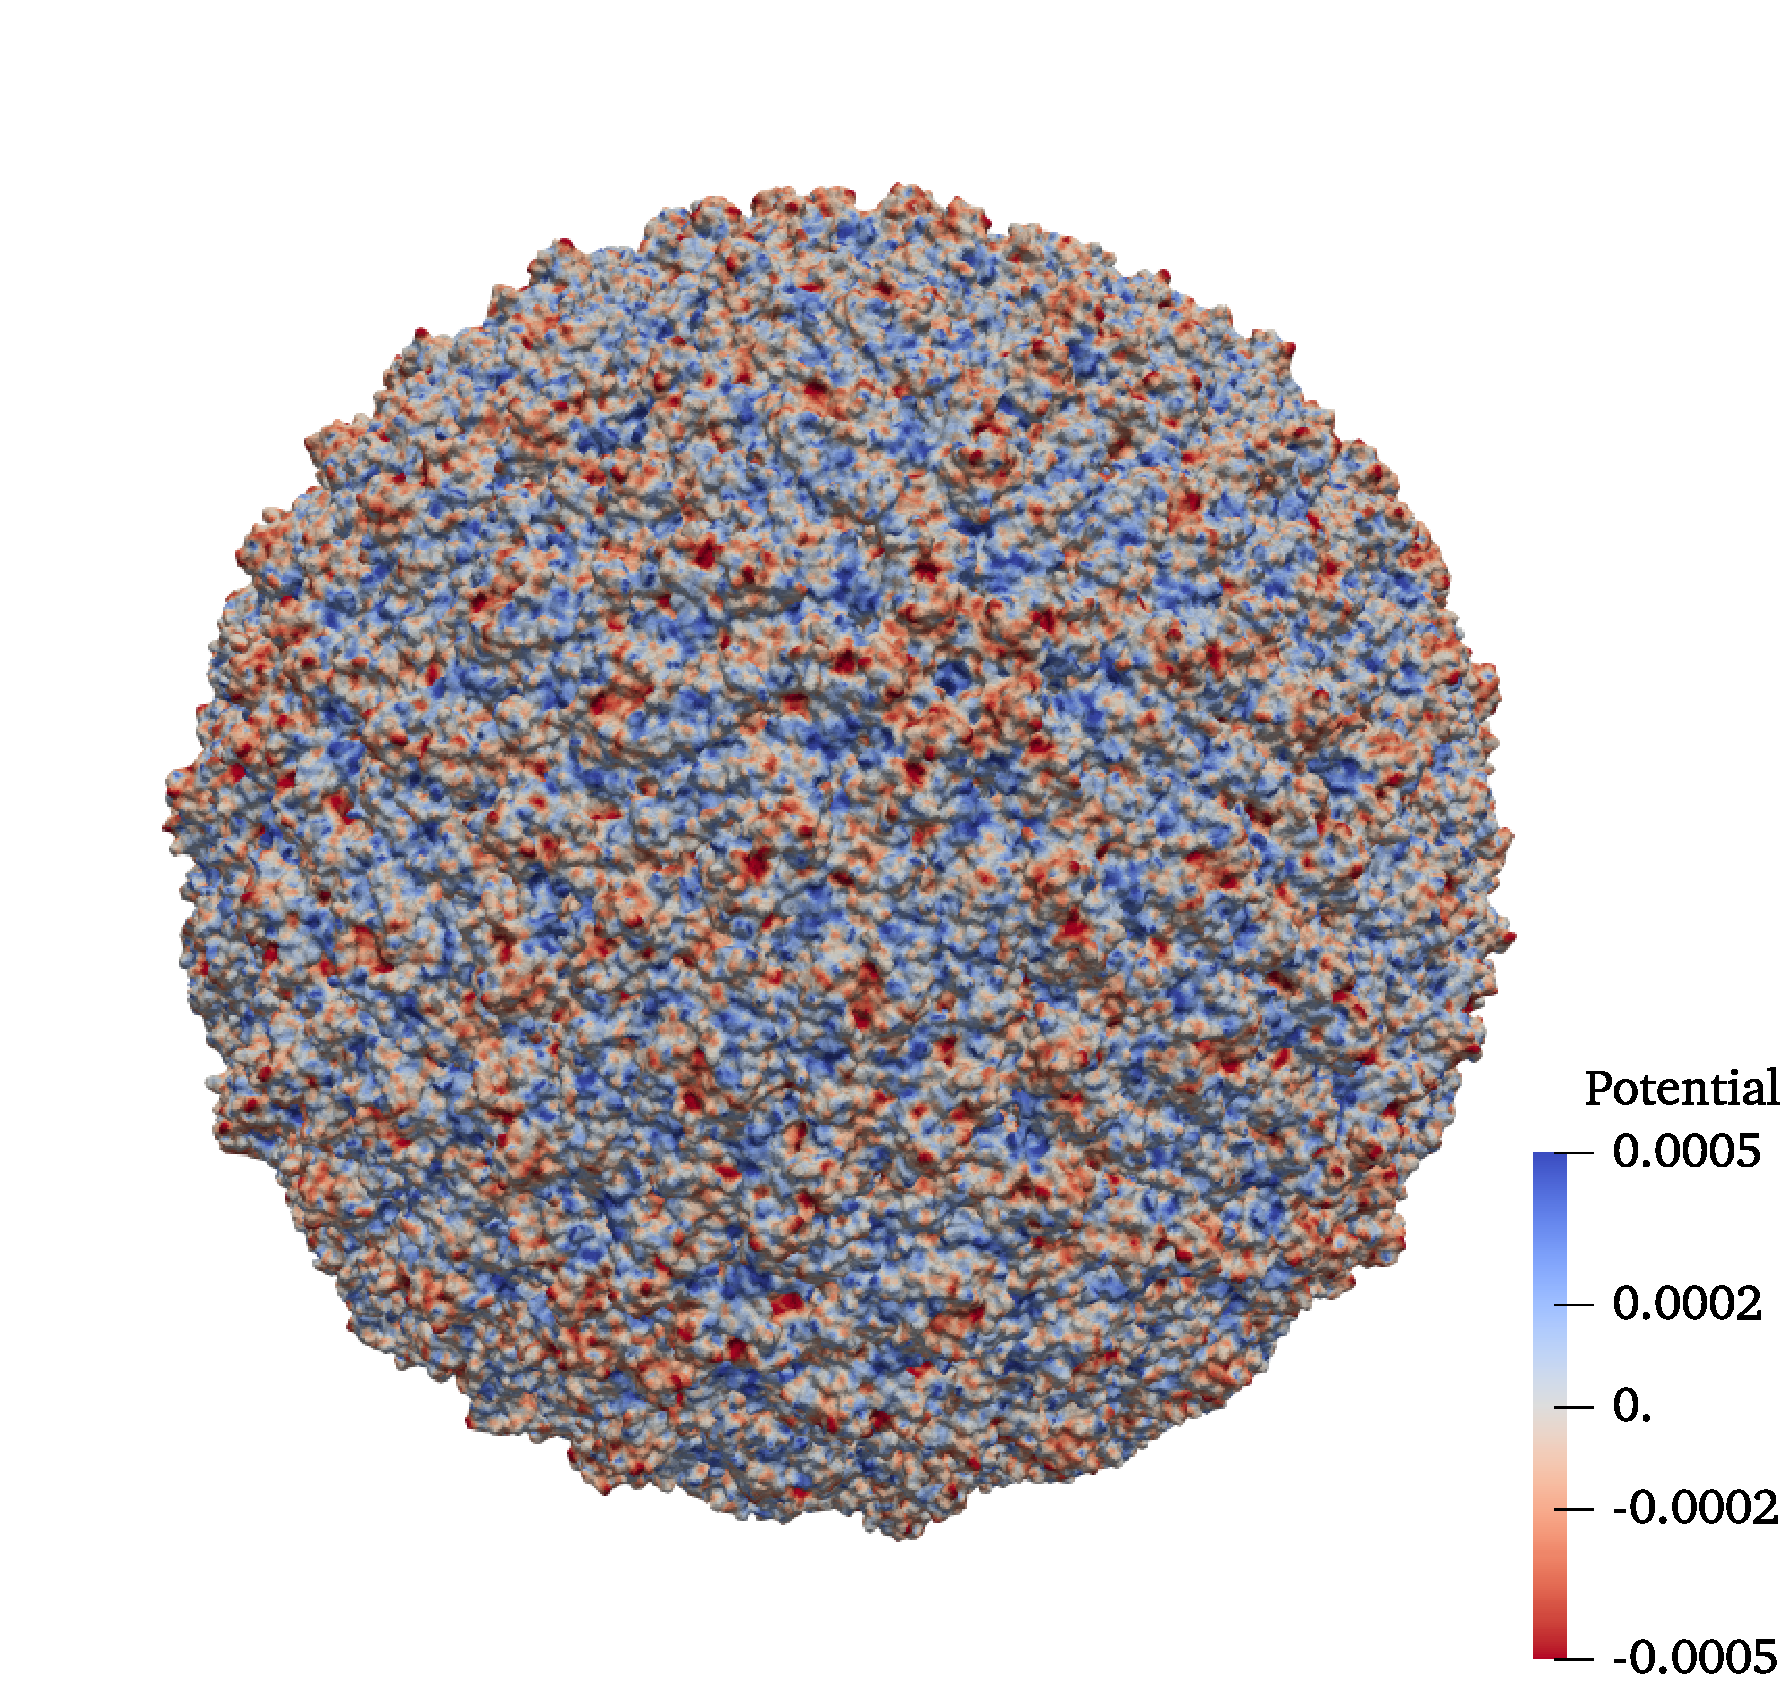
\includegraphics[width=\linewidth]{6CO8_potential.png} 
    \caption{Surface electrostatic potential of Zika virus. Visualization generated using ParaView.}
    \label{fig:6CO8_potential}
\end{figure*}

Table \ref{tab:6CO8_result} summarizes the results and performance.
Again, we confirmed that the derivative formulation yields a well-conditioned system, which converged in 18 iterations and took less than 1.5 hours to solve.
By contrast, direct formulation took almost twice as long to converge.

In this case, we also verified against \pygbe \cite{cooper2016pygbe}, a Python \bem library for biomolecular electrostatics.
Based on the solvation energy computed from \pygbe: $-117261.1$ [kcal/mol], the relative difference of our result is 0.6\% for direct formulation and 0.9\% for derivative formulation.
Figure \ref{fig:6CO8_potential} shows the computed electrostatic potential on the surface.

\subsection{Reproducibility package}

Besides releasing our code with an open-source license, we spared no effort to maximize the reproducibility of this work via a ``repro-pack" in a version-control repository.
It contains all raw data from the experiments and post-processing scripts, which are sufficient to produce every result presented in this section.
The ``repro-pack" also provides driver and utility scripts should readers be interested in running these cases on their own hardware.
The meshes and pqr files are available on Zenodo.

\section{Discussion} \label{sec:discussion}
%!TEX root = main.tex
With this paper, we introduce a new platform for computational investigations in biomolecular electrostatics, combining high-performance with high researcher productivity. 
Bempp-Exafmm integrates one of the most trusted boundary element software packages with one of the most performant fast-summation libraries using multipole methods. 
A Python entry point gives researchers ease of use, while enabling computational research at virus scale on standard workstations.
The software is open source under permissive public licenses, and developed in the open.

We present several results that confirm the usefulness of the platform, verify solution correctness with classic benchmarks, and showcase the performance. 
% conditioning
In section \ref{result_conditioning}, we compared the conditioning of the interior and exterior derivative formulations.
Despite the fact that both yield a well-conditioned system, where the condition number does not grow with the problem size, the exterior formulation always converges faster due to the closeness of its eigenvalues.
It shows a greater advantage over the interior formulation as the difference between $\epsilon_1$ and $\epsilon_2$ becomes larger.
This study also serves as example of how users can benefit from our high-productivity platform.
Through interactive computing, users can adapt various formulations, try out different problem setups, analyze intermediate results on-the-fly without the hassle of recompilation.

% mesh refinement
We performed two mesh refinement studies to verify Bempp-Exafmm, using a spherical molecule with an off-center charge and bovine pancreatic trypsin inhibitor.
In the former study, we compared with the analytical solution; in the latter, we compared with an approximate value from Richard extrapolation.
In both cases, we used the direct formulation and the exterior derivative formulation.
To reveal the discretization error, we set the \fmm expansion order to 10 to achieve 9 digits of accuracy.
The error of the computed solvation energy decays linearly with respect to $N$, as shown in Figure \ref{fig:sphere_convergence} and \ref{fig:5PTI_convergence}.

% performance and Zika virus
In section \ref{result_performance}, we elaborate on the performance of Bempp-Exafmm for different problem sizes using both formulations.
The linear complexity of the assembly time (Figure \ref{fig:sphere_assembly_time}) and \fmm time (Figure \ref{fig:sphere_fmm}) guarantees the overall linear time complexity of Bempp-Exafmm, which, together with the linear space complexity shown in Figure \ref{fig:sphere_memory}, makes it feasible to perform large-scale simulations on a workstation.
Table \ref{tab:sphere_time} lists the timings in detail.
Despite being ill-conditioned, the direct formulation still shows an advantage in terms of the overall time for smaller problem sizes.
Conversely, the derivative formulation shines in larger problems.
The crossover point should be problem- and hardware-specific.
Finally, we computed the solvation energy of Zika virus using both formulations and verified our results against PyGBe in \ref{result_zika}.
The linear system, for a mesh containing 10 million boundary elements, was solved in 80 minutes on a single node, which gives us confidence in the capability of Bempp-Exafmm of solving virus-scale problems.


A Poisson-Boltzmann solver is not something new in itself.
They have been around for decades, are available as stand-alone applications and web servers, and come in a variety of implementations, ranging from finite difference, to finite element, and boundary element methods.
Moreover, some are integrated into a number of computational workflows that use them for mean field potential visualization \cite{HumphreyETal1996} and free energy calculations \cite{MillerETal2012,KumariETal2014,WangETal2018}, usually interfaced through bash or Python scripts.

The modern design of Bempp is built such that high-performance computations are accessible from a high-productivity language.
This makes our effort stand out in the current landscape of Poisson-Boltzmann solvers in three ways: interoperability, ease of use, and robustness. 
\begin{enumerate}
\item Interoperability: Bempp is written in Python, and hence, is callable from a Jupyter notebook. This fits naturally in any computational workflow that uses Jupyter notebooks, for example, with openMM \cite{EastmanETal2017}, Biobb \cite{AndrioETal2019}, MDAnalysis \cite{GowersETal2019}, pytraj \cite{RoeCheatham2013}, or PyMOL \cite{PyMOL}. The Jupyter Notebook becomes a computational glue across models and scales; no interface script required. 

\item Ease of use: Python and Jupyter notebooks are widely used, even in non-computational settings. Bempp is easily installed through \texttt{conda}, and gives a result in less than 20 lines of code. This, moreover, using parallel and state-of-the-art algorithms in a way that is almost transparent to the user, allowing for large-scale simulations on workstations or small clusters at no extra cost.
Also, there is a thin layer between the application and Bempp, giving a more experienced user access to develop new models, for example, through the \fmm-\bem coupling capability of Bempp.

\item Robustness: Bempp is actively developed with high standards of software engineering, such as unit and system testing, continuous integration, etc. It was originally designed for scattering problems, impacting a large group of people, well beyond the molecular simulation community. This builds high trust and reliability of the code, as it is thoroughly tested in a diverse set of applications. The software has a better chance to survive in the long term, and any improvements done by people in other domains will have an effect on its use to solve the Poisson-Boltzmann equation. 

\end{enumerate}

Many popular molecular simulation software packages exist, designed for different applications, scales, quantities of interest, etc.
This has led to community-wide efforts, such as BioExcel and MolSSI, that are looking for a common ground between them, as well as promoting good software development practices for robust and easy-to-use codes.
This standard is very much aligned with our work.

\section*{Acknowledgments}
We thank Dr. Sergio Pantano for providing us with the parameterized structure of the Zika virus capsid.
C. Cooper’s work was supported by ANID through Basal FB0821.
The work from Timo Betcke was supported by Engineering and Physical Sciences Research Council Grant EP/V001531/1.

\bibliography{./reference}{}
\bibliographystyle{elsarticle-num}
\end{document}
